\documentclass[10pt]{article}
\usepackage{icmlko}

\icmlmeta{IP 파운데이션 월드모델}{8}{사람이 본 것을 문서는 말하지 않는다}{축을 문서에서 복원하면 승률 100\%가 5\%로 무너진다 --- 앵커 구조의 병목은 인코더였다}

\begin{document}

\twocolumn[
\icmlheader

\begin{abstract}
노트 7은 비대칭 하나를 발견하고 질문 하나를 남겼다. 앵커된 슬롯 구조에서 인코더는
비선형이어야 하고 헤드는 선형이어야 하는데, 그렇다면 선형 모델이 이기는 이유는
선형이어서인가 아니면 \emph{사람이 매긴 축을 그대로 받기 때문}인가. 이 노트가
답한다. 폴드 밖에서 문서 피처만으로 다섯 축을 예측하고 그 예측치로 결과를 맞히면,
\textbf{승률 100\%가 5\%로 무너진다}(차이 $-$0.0313 $\to$ $+$0.0254). 개별 축은
셋이 약하게나마 복원되는데도(타깃 폭 90\%, 입장 허들 100\%, 굿즈 규모 85\%) 합치면
신호가 사라진다 --- 복원 오차가 상관돼 선형 결합을 파괴한다. \textbf{사람 태그는
문서의 요약이 아니라 새 정보다.} 아이돌 도메인 조사가 같은 결론에 독립적으로
도달했다. 초동 라벨의 계수 기준을 출처와 분리해 한터 단독 풀을 67건에서 81건으로
회수한 뒤 다섯 축을 유도해 보니, \textbf{입장 허들과 굿즈 규모는 대응 필드가 아예
없다}(태깅률 0\%). 문서에서도 복원되지 않고 다른 도메인에는 필드도 없다면, 축은
수집해야 하는 대상이다. 부록에서 노트 5의 반복 CV 수치를 정정한다 --- 32개 변형
전수 비교 결과 결론을 정하는 요인은 레인 하나뿐이었다.
\end{abstract}
]

\section{남겨둔 질문}

노트 7의 마지막 절은 이렇게 끝났다.

\begin{quote}\fontsize{9.2}{11}\selectfont
ridge가 100\%로 이기는 이유가 선형이어서가 아니라 사람이 매긴 축을 그대로 받기
때문이라면, 앵커 구조의 병목은 헤드가 아니라 인코더다.
\end{quote}

이 구분은 사소하지 않다. 병목이 헤드면 구조를 고치면 되지만, 병목이 인코더면
\emph{데이터를 더 모아야} 한다. 그리고 어떤 데이터를 모아야 하는지도 달라진다 ---
문서를 더 모을 것인가, 사람 태그를 더 매길 것인가.

측정은 직접적이다. 폴드 밖에서 문서 피처만으로 각 축을 예측해 사람 태그와
대조하고, 그 예측치로 결과까지 맞혀 본다. 팝업 75건, IP 무작위 5폴드 20회 반복,
문서 피처 70개(다섯 축 태그 자신은 제외)를 쓴다.

\section{축은 부분적으로만 복원된다}

먼저 축 하나하나를 문서에서 얼마나 맞히는가.

\begin{table}[t]
\centering\tsize
\caption{문서 피처만으로 각 축을 예측. 비교 기준은 그 축의 폴드 내 중앙값이다.
음수가 상수보다 낫다는 뜻이다.}
\begin{tabular}{lrrr}
\toprule
축 & 상수 MAE & 최선 차이 & 이긴 비율 \\
\midrule
입장 허들   & 0.2533 & $-$0.0344 & 100\% \\
타깃 폭     & 0.2100 & $-$0.0092 & 90\% \\
굿즈 규모   & 0.2333 & $-$0.0140 & 85\% \\
\midrule
매장 노출도 & 0.1633 & $+$0.0011 & 35\% \\
미디어 투입 & 0.1900 & $+$0.0343 & 0\% \\
\bottomrule
\end{tabular}
\end{table}

\begin{figure}[t]
\centering
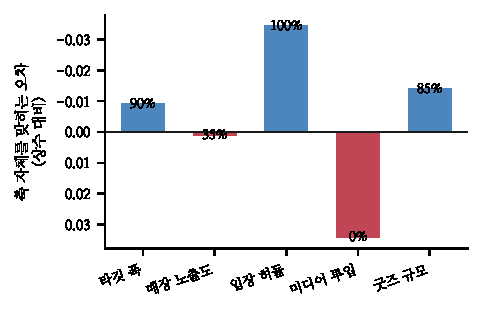
\includegraphics[width=\columnwidth]{figs/axis_recovery.pdf}
\caption{축별 복원 성적. 막대 옆 숫자는 20회 중 상수를 이긴 비율이다. 셋은
복원되고 둘은 되지 않는다.}
\end{figure}

셋은 복원된다. 특히 입장 허들은 20회 전부 이긴다 --- 예약 필요 여부나 대기 구조는
문서에 비교적 명시적으로 적히기 때문일 것이다. 반면 미디어 투입은 20회 중 0회로
상수보다 크게 나쁘다. 홍보 물량은 기획서에 숫자로 남지 않는다.

여기까지만 보면 절반의 성공처럼 보인다. 그런데 축은 따로 쓰는 물건이 아니다.

\section{합치면 무너진다}

복원한 다섯 축으로 결과를 예측한다. 비교 대상은 사람 태그를 그대로 쓴 경우다.
두 팔은 뒤쪽 모델도 폴드도 완전히 같고, 앞쪽 입력만 다르다.

\begin{table}[t]
\centering\tsize
\caption{2단 예측. IP 무작위 5폴드 20회 반복, 두 단 모두 ridge.}
\begin{tabular}{lrr}
\toprule
축의 출처 & 차이 중앙 & 이긴 비율 \\
\midrule
사람이 매긴 축       & $-$0.0313 & \textbf{100\%} \\
문서에서 복원한 축   & $+$0.0254 & \textbf{5\%} \\
\bottomrule
\end{tabular}
\end{table}

\begin{figure}[t]
\centering
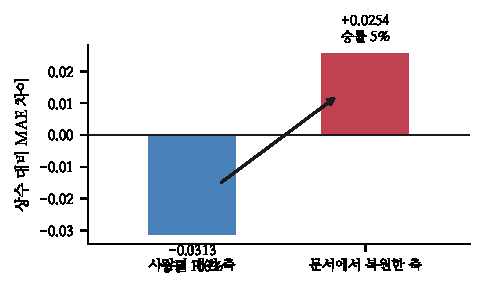
\includegraphics[width=\columnwidth]{figs/collapse.pdf}
\caption{같은 다섯 축, 같은 모델, 같은 폴드. 앞단만 사람에서 문서로 바꾸면
100\%가 5\%가 된다.}
\end{figure}

100\%에서 5\%다. 개별 축이 셋이나 복원됐는데도 합치면 상수보다 나빠진다.

이유는 오차의 상관이다. 각 축을 같은 문서 피처로 예측하면 복원 오차가 서로
독립이 아니다. 예컨대 규모가 큰 기획서는 모든 축을 동시에 높게 밀고, 작은
기획서는 동시에 낮게 민다. 그러면 복원된 다섯 축은 실질적으로 하나의 ``규모''
축으로 축퇴하고, 다섯 축이 서로 다른 것을 재기 때문에 생기던 이득이 사라진다.
개별 복원 성적이 좋아도 이 축퇴는 막지 못한다.

\claimx{다섯 축을 문서에서 복원해 결과를 예측하면 상수보다 나빠진다(승률 5\%).
사람 태그는 문서의 요약이 아니라 문서에 없는 정보를 담고 있다.}{복원된 다섯 축을
서로 직교화(잔차화)한 뒤에도 승률이 회복되지 않으면 원인은 축퇴가 아니라 정보
부족이다. 반대로 직교화만으로 회복되면 문서에 정보는 있고 추출이 잘못된 것이다.}

\section{아이돌 쪽에서 같은 결론이 나왔다}

같은 기간에 아이돌 도메인 데이터를 정비하다가 독립적으로 같은 벽에 부딪혔다.

\subsection{먼저 계수 기준을 분리했다}

아이돌 레코드 282건 중 175건에 초동 라벨이 있다. 그런데 \texttt{chodong\_basis}가
통제 어휘가 아니라 자유 텍스트였다. 175건의 값이 28가지로 흩어져 있었는데 그
대부분이 기준이 아니라 \emph{출처}였다 --- ``나무위키 앨범 문서 `초동 판매량'
전사표'' 같은 문자열이 통째로 들어가 있었다. 나무위키는 출처지 계수 기준이 아니다.

이것은 노트 1이 팝업에서 규명한 병과 정확히 같은 것이다. 거기서는 주최자 발표와
현장 계수가 한 컬럼에 섞여 2.75배 벌어져 있었다. 여기서는 한터와 써클과 오리콘이
섞여 있다. 셋은 집계 기간도 유통망도 다르므로 다른 물리량이다.

출처를 별도 필드로 옮기고 기준을 초동 전용 필드에서만 판정하도록 고쳤다.
처음에는 전체 노트를 훑었더니 33건이 ``복수 기준 언급''으로 판정 불가가 됐는데,
확인해 보니 전부 오탐이었다 --- ``써클차트 2019년 12주차 주간 앨범차트 최고 N위''
같은 문장은 초동 수치의 기준이 아니라 별개의 차트 순위 서술이다. 판정 범위를
좁히자 한터 단독 확정이 67건에서 \textbf{81건}으로 늘고 판정 불가는 33건에서
12건으로 줄었다. 반대 방향 오탐도 잡혔다(써클 15$\to$1).

\subsection{그리고 두 축의 데이터가 없었다}

이 81건에 팝업의 다섯 축을 매기려 했다. 소속사 체급은 손으로 등급을 매기지 않고
--- 그것은 내가 아는 것을 데이터에 주입하는 것이고 검정할 수 없다 --- 각 데뷔
시점보다 엄격히 이전의 같은 소속사 데뷔 실적으로 사전 통계를 만들었다.

\begin{figure}[t]
\centering
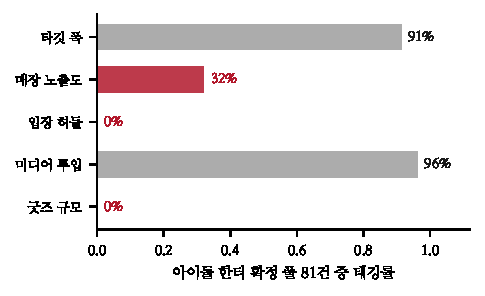
\includegraphics[width=\columnwidth]{figs/idol_cov.pdf}
\caption{아이돌 한터 확정 81건의 축 태깅률. 두 축은 대응 필드가 아예 없다.}
\end{figure}

\begin{table}[t]
\centering\tsize
\caption{아이돌 도메인의 축 대응물과 태깅률.}
\begin{tabular}{llr}
\toprule
축 & 아이돌 대응물 & 태깅률 \\
\midrule
미디어 투입 & 서바이벌·사전 화제·소속사 & 96\% \\
타깃 폭     & 성별 구성·인원·서바이벌 & 91\% \\
매장 노출도 & 소속사 사전 실적 & 32\% \\
\midrule
입장 허들   & 앨범 가격·진입 비용 & \textbf{0\%} \\
굿즈 규모   & 앨범 버전 수·특전 & \textbf{0\%} \\
\bottomrule
\end{tabular}
\end{table}

두 축은 태깅률이 0이다. 아이돌 레코드에 앨범 가격도 버전 수도 수집돼 있지 않다.
매장 노출도는 32\%인데, 표본의 소속사 대부분이 데뷔 한 건뿐이라 사전 실적이
없기 때문이다.

\claimx{팝업의 다섯 축은 현재 아이돌 데이터로 전이 실험을 할 수 없다. 둘은
태깅률이 0이고 하나는 32\%다.}{앨범 버전 수와 가격을 수집해 태깅률이 올라간 뒤에도
전이가 일어나지 않으면, 축이 도메인 불변이라는 가설 자체가 틀린 것이다.}

\section{그래서 축은 수집 대상이다}

두 결과가 한 방향을 가리킨다.

\begin{itemize}[leftmargin=1.1em,itemsep=0.15em]
\item 팝업에서 축은 \emph{문서로부터 복원되지 않는다}. 사람이 읽고 매겨야 한다.
\item 아이돌에서 축의 절반은 \emph{필드가 아예 없다}. 밖에서 가져와야 한다.
\end{itemize}

파운데이션 월드모델의 입력 설계가 바뀐다. 원래 그림은 도메인별 인코더가 원문서를
읽어 공유 슬롯으로 사상하는 것이었다. 그 그림은 인코더가 문서에서 축을 뽑아낼 수
있다는 전제 위에 서 있었고, 그 전제가 무너졌다.

수정된 그림에서 축은 \textbf{관측 대상}이다. 도메인마다 그 축을 재는 고유한
측정 경로가 있고, 인코더가 하는 일은 원문서 해석이 아니라 \emph{측정된 축을 공통
눈금으로 맞추는} 일이다.

\begin{itemize}[leftmargin=1.1em,itemsep=0.15em]
\item 굿즈 규모 --- 팝업: 굿즈 종류 수 / 아이돌: 앨범 버전 수, 특전 구성
\item 입장 허들 --- 팝업: 예약·대기 구조 / 아이돌: 앨범 가격, 팬덤 진입 비용
\item 매장 노출도 --- 팝업: 상권 등급 / 아이돌: 유통·음방 확보력
\end{itemize}

아이돌 쪽 두 축은 공개 데이터로 수집 가능하다. 음반 유통 상품 페이지에 버전 수와
정가가 그대로 있다 --- 예컨대 2026년 4월 데뷔한 한 그룹의 데뷔 앨범은 8종 세트
130,400원, 단품 16,300원으로 조회된다. 이것이 다음 수집 과제다.

\section{부록 --- 노트 5 반복 CV 수치 정정}

노트 7이 예고한 32개 변형 전수 비교가 끝났다. 피처 표현(원값 대 0--1 정규화),
마스크 컬럼 유무, 표본 가중치 유무, 레인, 피처 집합을 모두 교차했다.

결과는 단순했다. \textbf{결론을 정하는 요인은 레인 하나뿐이다.} 마스크와 정규화와
가중치는 넷째 자리에서만 움직인다.

\begin{table}[t]
\centering\tsize
\caption{32개 변형 중 대표값. 마스크·정규화·가중치를 어떻게 바꿔도 같은 값이 나온다.}
\begin{tabular}{llrr}
\toprule
피처 집합 & 레인 & 차이 중앙 & 이긴 비율 \\
\midrule
고정 5종 & ridge & $-$0.0354 & 100\% \\
기획 10종 & ridge & $-$0.0079 & 70\% \\
기획 10종 & 트리 & $+$0.0046 & 45\% \\
고정 5종 & 트리 & $+$0.0248 & 15\% \\
\bottomrule
\end{tabular}
\end{table}

노트 5는 기획 10종의 반복 CV를 차이 $-$0.0290, 승률 98\%로 보고했다. 재현되지
않는다. 저장된 구현으로 다시 재면 $-$0.0079, 70\%다. 노트 5의 실행은 인라인이라
코드가 남지 않았으므로 어느 지점이 달랐는지 특정할 수 없다. \textbf{재현 가능한
쪽 수치를 채택하고 노트 5의 해당 값을 정정한다.}

고정 5종은 노트 5($-$0.0442, 100\%)와 재현($-$0.0354, 100\%)이 부합하므로
그 결론은 유지된다. 그리고 이 정정은 노트 7의 결론을 오히려 강화한다 --- 다섯이
열보다 낫다는 격차가 보고된 것보다 크다.

\section{한계}

\begin{itemize}[leftmargin=1.1em,itemsep=0.15em]
\item 축 복원 실패가 ``문서에 정보가 없다''를 뜻하는지 ``내 피처화가 정보를
      못 담았다''를 뜻하는지 이 실험은 가르지 못한다. 문서 원문 임베딩으로
      다시 재야 한다.
\item 축퇴 가설(복원 오차가 상관돼 하나의 규모 축으로 무너진다)은 아직 직접
      검증하지 않았다. 반증 조건에 적은 직교화 실험이 다음이다.
\item 아이돌 축 유도는 규칙 기반이며 사람 태깅이 아니다. 팝업 쪽 태그와 같은
      물건이라는 보장이 없다.
\item 모든 반복 분할은 시간 순서를 쓰지 않는다. 안정성 판정용이다.
\end{itemize}

\section{다음}

\begin{enumerate}[leftmargin=1.3em,itemsep=0.15em]
\item 아이돌 앨범 버전 수·정가 수집 --- 81건. 두 축의 태깅률 0을 메운다.
\item 복원 축 직교화 실험 --- 축퇴 가설의 직접 검정.
\item 문서 원문 임베딩으로 축 복원 재시도 --- 피처화 탓인지 가른다.
\item 태그 순열 대조군 --- 노트 6이 남긴 반증 조건.
\end{enumerate}

\vspace{0.6em}
\hrule height 0.3pt
\vspace{0.5em}
{\footnotesize
\textbf{참고문헌}\\[0.3em]
Ben-David, S. et al. (2010). A theory of learning from different domains.
\emph{Machine Learning}, 79(1--2), 151--175.\\[0.15em]
Caruana, R. (1997). Multitask learning. \emph{Machine Learning}, 28(1), 41--75.\\[0.15em]
Kaufman, S., Rosset, S., Perlich, C. (2012). Leakage in data mining.
\emph{ACM TKDD}, 6(4), 1--21.\\[0.15em]
Standley, T. et al. (2020). Which tasks should be learned together in multi-task
learning? \emph{ICML 2020}, 9120--9132.
}

\end{document}
